\section{Ćwiczenia 10: 11-V-2017}
\subsection{Zadania domowe A}
\paragraph{A1} Rozważmy dwa łańcuchy Markowa, $L_1$ i $L_2$, których stanami jest pięć zbiorów niezależnych ścieżki na trzech wierzchołkach (jeden zbiór pusty, trzy jednoelementowe i jeden dwuelementowy).
\begin{itemize}
\item Zasady przejścia dla łańcucha $L_1$ są następujące:
\begin{itemize}
\item Mając zbiór niezależny $I$, rzuć moneta.
\item Jeśli wypadł orzeł, to wylosuj jeden z trzech wierzchołków $v$, każdy z jednakowym prawdopodobieństwem. Gdy $v \not \in I$ i $I \cup \{v\}$ jest niezależny, wtedy zamień $I$ na $I \cup \{v\}$; w przeciwnym przypadku zostań w $I$.
\item Jeśli wypadła reszka, to wylosuj jeden z trzech wierzchołków $v$, każdy z jednakowym prawdopodobieństwem. Gdy $v \in I$, wtedy zamień $I$ na $I \setminus v$; w przeciwnym przypadku zostań w $I$.
\end{itemize}
\item  Zasady przejścia dla łańcucha $L_2$ są takie:
\begin{itemize}
\item  Mając zbiór niezależny $I$, rzuć monetą.
\item Jeśli wypadł orzeł i istnieje przynajmniej jeden taki zbiór niezależny $J$, że $J \supset  I$ i $|J \setminus I| = 1$, wybierz losowo jeden z takich zbiorów (każdy z jednakowym prawdopodobieństwem) i zamień $I$ na $J$.
\item Jeśli wypadła reszka i istnieje przynajmniej jeden taki zbiór niezależny $J$, że $J \subset I$ i $|I \setminus J| = 1$, wybierz losowo jeden z takich zbiorów (każdy z jednakowym prawdopodobieństwem) i zamień $I$ na $J$.
\item W pozostałych przypadkach zostań w $I$.
\end{itemize}
\end{itemize}
\begin{enumerate}[label=\alph*)]
\item Oceń intuicyjnie, czy rozkłady stacjonarne dla $L_1$ i $L_2$ są takie same.
\begin{comment}
\begin{multicols}{2}
[Oznaczenia: Moneta - $\rightarrow$ rzut monetą\\
O $\rightarrow$  Orzeł, R $\rightarrow$ Reszka\\
ind. $\rightarrow$ niezależny]
% Define block styles
\tikzstyle{decision} = [diamond, draw, text badly centered, node distance=2cm, inner sep=0pt]
\tikzstyle{block} = [rectangle, draw, text centered, rounded corners, minimum height=1em,node distance=2.5cm]
\tikzstyle{line} = [draw,->,ultra thick]
Pierwszy\\
\begin{tikzpicture}
\node[block] (init) {I};
\node[decision, below of=init] (moneta) {Mon};
\node[block, below left of=moneta,text width=5em] (or) {O\newline $\exists _J J\supset I \land |J\setminus I|=1$};
\node[block, below right of=moneta,text width=7em] (re) {R\newline $\exists _J J \text{ind. } \land J\subset I \land |I\setminus J|=1$};
\node[block, left of=init] (or2) {$I:=J$};
\node[block, right of=init] (re2) {$I:=J$};

\path[line] (init) -- (moneta);
\path[line] (moneta) -- (or);
\path[line] (moneta) -- (re);
\path[line] (moneta) -- node [left,near start] {$\sfrac{1}{2}$} (or);
\path[line] (moneta) -- node [right,near start] {$\sfrac{1}{2}$} (re);
\path[line] (or) -- node [left,near start] {tak} (or2);
\path[line] (re) -- node [right,near start] {tak} (re2);
\path[line] (or2) -- (init);
\path[line] (re2) -- (init);
\end{tikzpicture}

Drugi\\
\begin{tikzpicture}
\node[block] (init) {I};
\node[decision, below of=init] (moneta) {Mon};
\node[decision, below left of=moneta,text width=1em] (or) {O: $v$};
\node[decision, below right of=moneta,text width=1em] (re) {R: $v$};
\node[block, below of=or] (or2) {$v\not\in I \land I\cup \{v\} \text{ind. }$};
\node[block, below of=re] (re2) {$v\in I$};
\node[block, left of=init] (or3) {$I:= I\cup \{v\}$};
\node[block, right of=init] (re3) {$I:= I\setminus \{v\}$};

\path[line] (init) -- (moneta);
\path[line] (moneta) -- (or);
\path[line] (moneta) -- (re);
\path[line] (moneta) -- node [left,near start] {$\sfrac{1}{2}$} (or);
\path[line] (moneta) -- node [right,near start] {$\sfrac{1}{2}$} (re);
\path[line] (or) -- node [left,near start] {$\sfrac{1}{3}$} (or2);
\path[line] (re) -- node [right,near start] {$\sfrac{1}{3}$} (re2);
\path[draw,->,bend left,ultra thick] (re2) node [near start] {tak} (re3);
\path[line] (or2) -- node [near start] {tak} (or3);
\path[line] (re2) -- node [near start] {nie} (init);
\path[line] (or2) -- node [near start] {nie} (init);
\path[line] (or3) -- (init);
\path[line] (re3) -- (init);
\end{tikzpicture}
\end{multicols}
\end{comment}

Nie, nie są gdyż są inne warunki przejścia itp.

\item Sprawdź swoje przypuszczenie, budując macierze przejścia i licząc rozkłady stacjonarne dla obu łańcuchów.

\textbf{Ile zbiorów tyle stanów!!}
\begin{figure}[H]
\centering
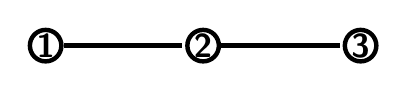
\begin{tikzpicture}[shorten >=1pt, auto, node distance=3cm, ultra thick,main node/.style={circle,draw,minimum size=.4cm,inner sep=0pt}]
\begin{scope}[every node/.style={font=\sffamily\large\bfseries}]
\node [main node](v1) at (0,0) {1};
\node [main node](v2) at (2,0) {2};
\node [main node](v3) at (4,0) {3};
\end{scope}
\path 
	(v1) edge (v2)
    (v2) edge (v3)
         ;
\end{tikzpicture}
\end{figure}
Ważne słowo - \textbf{niezależny} czyli bez połączeń krawędziami!\\
Stany $S=\{\{\emptyset\},\{\emptyset,1\},\{\emptyset,2\},\{\emptyset,3\},\{\emptyset,1,3\} \}$
\begin{enumerate}
\item $L_1$
\begin{align*}
\{\emptyset\}\rightarrow \{\emptyset\} &=\frac{1}{2} &&\text{Reszka potem 1,2,3}\\
\{\emptyset\}\rightarrow \{1\} &=\frac{1}{2}*\frac{1}{3}=\frac{1}{6} &&\text{Orzeł potem 1}\\
\{\emptyset\}\rightarrow \{2\} &=\frac{1}{2}*\frac{1}{3}=\frac{1}{6} &&\text{Orzeł potem 2}\\
\{\emptyset\}\rightarrow \{3\} &=\frac{1}{2}*\frac{1}{3}=\frac{1}{6} &&\text{Orzeł potem 3}\\
\{\emptyset\}\rightarrow \{1,3\} &=0 &&\text{Nie da się}\\
\{1\}\rightarrow \{\emptyset\} &= \frac{1}{2}*\frac{1}{3}=\frac{1}{6}&&\text{Reszka potem 1}\\
\{1\}\rightarrow \{1\} &= \frac{1}{2}*\frac{2}{3}+\frac{1}{2}*\frac{2}{3}=\frac{2}{3}&&\text{Orzeł potem 1,2 i Reszka potem 2,3}\\
\{1\}\rightarrow \{2\} &= 0&&\text{Nie da się}\\
\{1\}\rightarrow \{3\} &= 0&&\text{Nie da się}\\
\{1\}\rightarrow \{1,3\} &= \frac{1}{2}*\frac{1}{3}=\frac{1}{6} &&\text{Orzeł potem 3}\\
\{2\}\rightarrow \{\emptyset\} &= \frac{1}{2}*\frac{1}{3}=\frac{1}{6} &&\text{Reszka potem 2}\\
\{2\}\rightarrow \{1\} &= 0&&\text{Nie da się}\\
\{2\}\rightarrow \{2\} &= \frac{1}{2}*\frac{3}{3}+\frac{1}{2}*\frac{2}{3}=\frac{5}{6}&&\text{Orzeł potem 1,2,3 i Reszka potem 1,3}\\
\{2\}\rightarrow \{3\} &=0 &&\text{Nie da się}\\
\{2\}\rightarrow \{1,3\} &=0 &&\text{Nie da się}\\
\{3\}\rightarrow \{\emptyset\} &=\frac{1}{2}*\frac{1}{3}=\frac{1}{6} &&\text{Reszka potem 3}\\
\{3\}\rightarrow \{1\} &=0 &&\text{Nie da się}\\
\{3\}\rightarrow \{2\} &=0 &&\text{Nie da się}\\
\{3\}\rightarrow \{3\} &=\frac{1}{2}*\frac{2}{3}+\frac{1}{2}*\frac{2}{3}=\frac{2}{3} &&\text{Orzeł potem 2,3 i Reszka potem 1,2}\\
\{3\}\rightarrow \{1,3\} &=\frac{1}{2}*\frac{1}{3}=\frac{1}{6} &&\text{Orzeł potem 1}\\
\{1,3\}\rightarrow \{\emptyset\} &=0 &&\text{Nie da się}\\
\{1,3\}\rightarrow \{1\} &=\frac{1}{2}*\frac{1}{3}=\frac{1}{6} &&\text{Reszka potem 3}\\
\{1,3\}\rightarrow \{2\} &=0 &&\text{Nie da się}\\
\{1,3\}\rightarrow \{3\} &=\frac{1}{2}*\frac{1}{3}=\frac{1}{6} &&\text{Reszka potem 1}\\
\{1,3\}\rightarrow \{1,3\} &=\frac{1}{2}*\frac{3}{3}+\frac{1}{2}*\frac{1}{3} = \frac{4}{6}&&\text{Orzeł potem 1,2,3 i Reszka potem 2}
\end{align*}
\begin{figure}[H]
\centering
\begin{tikzpicture}[shorten >=1pt, auto, node distance=3cm, ultra thick,main node/.style={circle,draw,minimum size=.6cm,inner sep=0pt}]
\begin{scope}[every node/.style={font=\sffamily\large\bfseries}]
\node [main node](v1) at (3,0) {$\{\emptyset\}$};
\node [main node](v2) at (0,-1) {$\{1\}$};
\node [main node](v3) at (4,2) {$\{2\}$};
\node [main node](v4) at (-2.5,2) {$\{3\}$};
\node [main node](v5) at (-1,3) {$\{1,3\}$};
\end{scope}
\path 
	(v1) edge [loop below] node {$\sfrac{1}{2}$} (v1)
    	 edge [->,bend left] node[near start] {$\sfrac{1}{6}$} (v2)
         edge [->,bend left] node[near start] {$\sfrac{1}{6}$} (v3)
         edge [->,bend left] node[near start] {$\sfrac{1}{6}$} (v4)
    (v2) edge [loop left] node {$\sfrac{2}{3}$} (v2)
    	 edge [->,bend left] node[near start] {$\sfrac{1}{6}$} (v1)
         edge [->,bend left] node[near start] {$\sfrac{1}{6}$} (v5)
    (v3) edge [loop right] node {$\sfrac{5}{6}$} (v3)
    	 edge [->,bend left] node[near start] {$\sfrac{1}{6}$} (v1)
    (v4) edge [loop left] node {$\sfrac{2}{3}$} (v4)
    	 edge [->] node[near start] {$\sfrac{1}{6}$} (v1)
         edge [->,bend left] node[near start] {$\sfrac{1}{6}$} (v5)
    (v5) edge [->,bend left] node[near start] {$\sfrac{1}{6}$} (v1)
         edge [->,bend left] node[near start] {$\sfrac{1}{6}$} (v3)
         edge [->,bend left] node[near start] {$\sfrac{2}{3}$} (v4)
         ;
\end{tikzpicture}
\end{figure}
$$\mathbb{P}_{L_1}=\bbordermatrix{
&\{\emptyset\}&\{1\}&\{2\}&\{3\}&\{1,3\} \cr
\{\emptyset\} & \sfrac{1}{2} & \sfrac{1}{6} & \sfrac{1}{6} & \sfrac{1}{6} & 0 \cr
\{1\} & \sfrac{1}{6} & \sfrac{2}{3} & 0 & 0 & \sfrac{1}{6}  \cr
\{2\} & \sfrac{1}{6} & 0 & \sfrac{5}{6} & 0 & 0  \cr
\{3\} & \sfrac{1}{6} & 0 & 0 & \sfrac{2}{3} & \sfrac{1}{6}  \cr
\{1,3\} & 0 & \sfrac{1}{6} & 0 & \sfrac{1}{6} & \sfrac{4}{6} \cr
}$$
Rozkład stacjonarny:
\begin{align*}
&\bar{\pi}\mathbb{P}_{L_1}=\bar{\pi}\\
&\left[\pi _1,\pi _2,\pi _3,\pi _4,\pi _5,\right]\begin{bmatrix}
\sfrac{1}{2} & \sfrac{1}{6} & \sfrac{1}{6} & \sfrac{1}{6} & 0\\
\sfrac{1}{6} & \sfrac{2}{3} & 0 & 0 & \sfrac{1}{6}  \\
\sfrac{1}{6} & 0 & \sfrac{5}{6} & 0 & 0  \\
\sfrac{1}{6} & 0 & 0 & \sfrac{2}{3} & \sfrac{1}{6}  \\
0 & \sfrac{1}{6} & 0 & \sfrac{1}{6} & \sfrac{4}{6}
\end{bmatrix}=\left[\pi _1,\pi _2,\pi _3,\pi _4,\pi _5,\right]\\
&\left\{\begin{matrix}
\frac{1}{2} \pi _1+\frac{1}{6} \pi_2+\frac{1}{6} \pi _3 +\frac{1}{6} \pi _4 &= \pi _1\\
\frac{1}{6} \pi _1+\frac{2}{3} \pi _2+\frac{1}{6} \pi _5 &= \pi _2\\
\frac{1}{6} \pi _1+\frac{5}{6} \pi _3 &= \pi _3\\
\frac{1}{6} \pi _1+\frac{2}{3} \pi _4+\frac{1}{6} \pi _5 &= \pi _4\\
\frac{1}{6} \pi _2+\frac{1}{6} \pi _4+\frac{2}{3} \pi _5 &= \pi _5
\end{matrix}\right. \Leftrightarrow \left\{\begin{matrix}
\frac{1}{6} \pi_2+\frac{1}{6} \pi _3 +\frac{1}{6} \pi _4 & = \frac{1}{2}\pi _ 1\\
\frac{1}{6} \pi _1+\frac{1}{6} \pi _5 &= \frac{1}{3}\pi _2\\
\frac{1}{6} \pi _1&=\frac{1}{6} \pi _3\\
\frac{1}{6} \pi _1+\frac{1}{6} \pi _5 &=\frac{1}{3} \pi _4\\
\frac{1}{6} \pi _2+\frac{1}{6} \pi _4 &= \frac{1}{3}\pi _5
\end{matrix}\right. \Leftrightarrow \\
&\Leftrightarrow \left\{\begin{matrix}
\pi _1 &= \pi _2\\
\pi _1 &= \pi _3\\
\pi _1 &= \pi _4 \\
\pi _1 &= \pi _5 
\end{matrix}\right.\\
&\pi _1+\pi _2+\pi _3+\pi _4+\pi _5=1\Leftrightarrow 5\pi _1 = 1 \Leftrightarrow \pi _1 = \frac{1}{5}\\
&\bar{\pi}=\left[\frac{1}{5},\frac{1}{5},\frac{1}{5},\frac{1}{5},\frac{1}{5}\right]
\end{align*}

\item $L_2$\\
\textbf{Uwaga!} zbiór pusty jest podzbiorem dowolnego zbioru\\
Pamiętajmy, że $\{1\} \subset \{1\}$\\
Stany $S=\{\{\emptyset\},\{\emptyset,1\},\{\emptyset,2\},\{\emptyset,3\},\{\emptyset,1,3\} \}$

\begin{align*}
\{\emptyset\}\rightarrow \{\emptyset\} &= \frac{1}{2} &&\text{Reszka}\\
\{\emptyset\}\rightarrow \{1\} &= \frac{1}{2}*\frac{1}{3}=\frac{1}{6} &&\text{Orzeł potem zbiór 1 (z trzech)}\\
\{\emptyset\}\rightarrow \{2\} &= \frac{1}{2}*\frac{1}{3}=\frac{1}{6}&&\text{Orzeł potem zbiór 2 (z trzech)}\\
\{\emptyset\}\rightarrow \{3\} &= \frac{1}{2}*\frac{1}{3}=\frac{1}{6}&&\text{Orzeł potem zbiór 3 (z trzech)}\\
\{\emptyset\}\rightarrow \{1,3\} &= 0 &&\text{Zdarzenie niemożliwe}\\
\{1\}\rightarrow \{\emptyset\} &= \frac{1}{2}*1=\frac{1}{2} &&\text{Reszka potem zbiór 0 }\\
\{1\}\rightarrow \{1\} &=0 &&\text{Nie spełnia warunków Orła i Reszki}\\
\{1\}\rightarrow \{2\} &=0 &&\text{Nie spełnia warunków Orła i Reszki}\\
\{1\}\rightarrow \{3\} &=0 &&\text{Nie spełnia warunków Orła i Reszki}\\
\{1\}\rightarrow \{1,3\} &= \frac{1}{2}*1=\frac{1}{2}&&\text{Orzeł potem zbiór 1,3}\\
\{2\}\rightarrow \{\emptyset\} &=\frac{1}{2}*1=\frac{1}{2} &&\text{Reszka potem zbiór pusty}\\
\{2\}\rightarrow \{1\} &=0 &&\text{Zdarzenie niemożliwe}\\
\{2\}\rightarrow \{2\} &=\frac{1}{2} &&\text{Orzeł}\\
\{2\}\rightarrow \{3\} &=0 &&\text{Zdarzenie niemożliwe}\\
\{2\}\rightarrow \{1,3\} &=\frac{1}{8} &&\text{Nie spełnia warunków Orła i Reszki}\\
\{3\}\rightarrow \{\emptyset\} &=\frac{1}{2}*1=\frac{1}{2} &&\text{Reszka potem zbiór 0}\\
\{3\}\rightarrow \{1\} &=0 &&\text{Nie spełnia warunków Orła i Reszki}\\
\{3\}\rightarrow \{2\} &=0 &&\text{Nie spełnia warunków Orła i Reszki}\\
\{3\}\rightarrow \{3\} &=0 &&\text{Nie spełnia warunków Orła i Reszki}\\
\{3\}\rightarrow \{1,3\} &=\frac{1}{2}*1=\frac{1}{2} &&\text{Orzeł potem zbiór 1,3}\\
\{1,3\}\rightarrow \{\emptyset\} &=0 &&\text{Nie spełnia warunków Orła i Reszki}\\
\{1,3\}\rightarrow \{1\} &=\frac{1}{2}*1=\frac{1}{2}  &&\text{Reszka potem zbiór 1}\\
\{1,3\}\rightarrow \{2\} &=0 &&\text{Nie spełnia warunków Orła i Reszki}\\
\{1,3\}\rightarrow \{3\} &=\frac{1}{2}*1 &&\text{Reszka potem zbiór 3}\\
\{1,3\}\rightarrow \{1,3\} &=0 &&\text{Nie spełnia warunków Orła i Reszki}
\end{align*}
$$\mathbb{P}_{L_1}=\bbordermatrix{
&\{\emptyset\}&\{1\}&\{2\}&\{3\}&\{1,3\} \cr
\{\emptyset\} & \sfrac{1}{2} & \sfrac{1}{6} & \sfrac{1}{6} & \sfrac{1}{6} & 0 \cr
\{1\} & \sfrac{1}{2} & 0 & 0 & 0 & \sfrac{1}{2} \cr
\{2\} & \sfrac{1}{2} & 0 & \sfrac{1}{2} & 0 & 0  \cr
\{3\} & \sfrac{1}{2} & 0 & 0 & 0 & \sfrac{1}{2} \cr
\{1,3\} & 0 & \sfrac{1}{2} & 0 & \sfrac{1}{2} & 0 \cr
}$$
\begin{figure}[H]
\centering
\begin{tikzpicture}[shorten >=1pt, auto, node distance=3cm, ultra thick,main node/.style={circle,draw,minimum size=.6cm,inner sep=0pt}]
\begin{scope}[every node/.style={font=\sffamily\large\bfseries}]
\node [main node](v1) at (-1,-1.5) {$\{\emptyset\}$};
\node [main node](v2) at (3.5,-1.5) {$\{1\}$};
\node [main node](v3) at (3.5,3.5) {$\{2\}$};
\node [main node](v4) at (-2.5,1.5) {$\{3\}$};
\node [main node](v5) at (-1,3) {$\{1,3\}$};
\end{scope}
\path 
	(v1) edge [loop left] node {$\sfrac{1}{2}$} (v1)
    	 edge [->,bend left] node[near start] {$\sfrac{1}{6}$} (v2)
         edge [->,bend left] node[near start] {$\sfrac{1}{6}$} (v3)
         edge [->,bend left] node[near start] {$\sfrac{1}{6}$} (v4)
    (v2) edge [->,bend left] node[near start] {$\sfrac{1}{2}$} (v1)
         edge [->,bend left] node[near start] {$\sfrac{1}{2}$} (v5)
    (v3) edge [->,bend left] node[near start] {$\sfrac{1}{2}$} (v1)
    	 edge [->,bend left] node[near start] {$\sfrac{1}{2}$} (v3)
    (v4) edge [->,bend left] node[near start] {$\sfrac{1}{2}$} (v1)
         edge [->,bend left] node[near start] {$\sfrac{1}{2}$} (v5)
    (v5) edge [->,bend left] node[near start] {$\sfrac{1}{2}$} (v2)
         edge [->,bend left] node[near start] {$\sfrac{1}{2}$} (v4)
         ;
\end{tikzpicture}
\end{figure}
Rozkład stacjonarny:
\begin{align*}
&\bar{\pi}\mathbb{P}_{L_1}=\bar{\pi}\\
&\left[\pi _1,\pi _2,\pi _3,\pi _4,\pi _5,\right]\begin{bmatrix}
\sfrac{1}{2} & \sfrac{1}{6} & \sfrac{1}{6} & \sfrac{1}{6} & 0 \\
\sfrac{1}{2} & 0 & 0 & 0 & \sfrac{1}{2} \\
\sfrac{1}{2} & 0 & \sfrac{1}{2} & 0 & 0  \\
\sfrac{1}{2} & 0 & 0 & 0 & \sfrac{1}{2} \\
0 & \sfrac{1}{2} & 0 & \sfrac{1}{2} & 0 
\end{bmatrix}=\left[\pi _1,\pi _2,\pi _3,\pi _4,\pi _5,\right]\\
&\left\{\begin{matrix}
\frac{1}{2}\pi _1 + \frac{1}{2}\pi _2+ \frac{1}{2}\pi _3+ \frac{1}{2}\pi _4 &= \pi _1\\
\frac{1}{6}\pi _1 + \frac{1}{2}\pi _5 &= \pi _2\\
\frac{1}{6}\pi _1 + \frac{1}{2}\pi _3 &= \pi _3\\
\frac{1}{6}\pi _1 + \frac{1}{2}\pi _5 &= \pi_4 \\
\frac{1}{2}\pi _2+\frac{1}{2}\pi _4 &= \pi _5
\end{matrix}\right. \Leftrightarrow \left\{\begin{matrix}
\pi _1 &= 3x\\
\pi _2 &= x\\
\pi _3 &= x\\
\pi _4 &= x\\
\pi _5 &= x
\end{matrix}\right.\\
&\bar{\pi}=\left[\frac{3}{7},\frac{1}{7},\frac{1}{7},\frac{1}{7},\frac{1}{7}\right]
\end{align*}
\end{enumerate}
\end{enumerate}



\paragraph{A2} Opisz zwięźle ideę algorytmu, generującego losowy zbiór niezależny w grafie (w tym zbiór pusty) w taki sposób, że \label{par:10-A2}

\begin{enumerate}[label=\alph*)]
\item  w rozkładzie stacjonarnym dla tego procesu wszystkie podzbiory są jednakowo prawdopodobne.

\begin{enumerate}[label=\arabic*.]
\item Startujemy od zbioru pustego $I=\emptyset $
\item Rzucamy monetą taką, że $\mathsf{Pr}(O)=p$ a $\mathsf{Pr}(R)=1-\mathsf{Pr}(O)=1-p$
\item Wybieramy losowo wierzchołek $v$ w grafie $G$,
\item Jeśli 
\begin{itemize}
\item[] wypadł \textbf{O}rzeł i $I=I\cup \{v\}$ jest niezależny to\\
$I:=I\cup \{v\}$
\item[] wypadła \textbf{R}eszka i $v\in I$ to\\
$I:=I- \{v\}$
\end{itemize}
\item wracamy do punktu 2.
\end{enumerate}
\textbf{Odpowiedź: }uzyskamy gdy za $p$ podstawimy $\frac{1}{2}$ - wtedy uzyskamy ergodyczny Łańcuch Markowa - nie jest okresowy i jest nieprzywiedlny.
\begin{figure}[H]
\centering
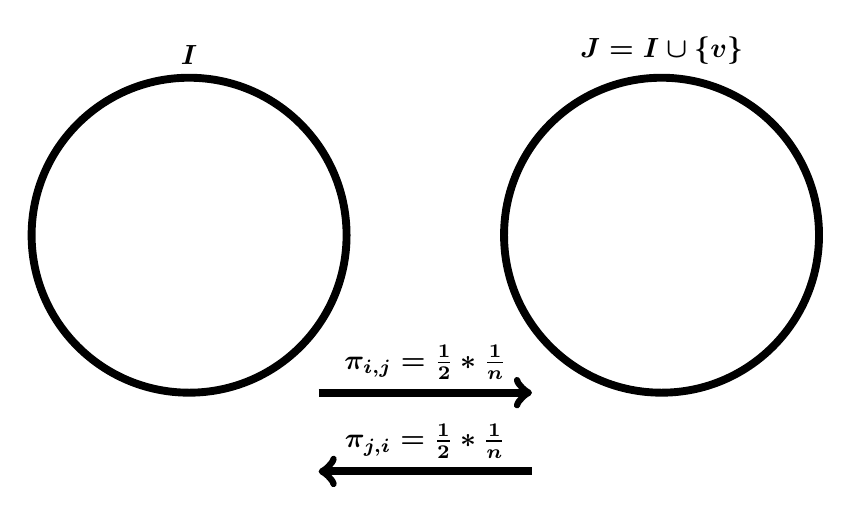
\begin{tikzpicture}[font=\boldmath,ultra thick,]
\draw[solid, line width=1mm]  (0,0) ellipse (2 and 2) node [above=2cm] {$I$};
\draw[solid, line width=1mm]  (6,0) ellipse (2 and 2) node [above=2cm] {$J=I\cup \{v\}$};
\node (v1) at (1.5,-2) {};
\node (v2) at (4.5,-2) {};
\node (v3) at (1.5,-3) {};
\node (v4) at (4.5,-3) {};
\draw[->,solid,line width=1mm,fill=black]  (v1) edge node [above] {$\pi _{i,j}=\frac{1}{2}*\frac{1}{n}$} (v2);
\draw[->,solid,line width=1mm,fill=black]  (v4) edge node [above] {$\pi _{j,i}=\frac{1}{2}*\frac{1}{n}$}(v3);
\end{tikzpicture}
\caption*{$\frac{1}{n}$ $\rightarrow$ wybranie 1 z $n$ wierzchołków\\$\frac{1}{2}$ $\rightarrow$ \textbf{O}rzeł albo \textbf{R}eszka\\Dowód okresowości - można wrócić z każdego stanu $I$ do każdego stanu $J$ i vice versa oraz nieprzywiedlności - z każdego okresu można się dostać w naturalnej liczbie kroków.}
\end{figure}
Więc dla $$\lim _{n\to\infty}\pi _{i,j}(n)=\pi _j$$ Co więcej dla dowolnej pary stanów $i,j\in S$ otrzymujemy $\pi_{i,j}=\pi _{j,i}$ więc $$\bar{\pi}=\left[\frac{1}{|S|},\frac{1}{|S|},...,\frac{1}{|S|}\right]$$

\item po wielu krokach otrzymamy każdy podzbiór niezależny z prawdopodobieństwem w przybliżeniu jednakowym.

\textbf{Odpowiedź: }Analogicznie jak w przykładzie powyżej, jednakże dla $p= \frac{1}{2}$ analogicznie jak wyżej rozkład po wielu ktokach będzie rozkładem stacjonarnym jak w podpunkcie a).
\item w rozkładzie stacjonarnym dla tego procesu każdy ze zbiorów niezależnych $A$ występuje z prawdopodobieństwem, 
$$\frac{2^{|A|}}{\sum _Z2^{|Z|}}$$
gdzie suma w mianowniku przebiega wszystkie zbiory niezależne grafu (w tym zbiór pusty).

\textbf{Odpowiedź: } Zgodnie z modyfikacją algorytmu: 
\begin{enumerate}[label=\arabic*.]
\item Startujemy od zbioru pustego $I=\emptyset $
\item Rzucamy monetą taką, że $\mathsf{Pr}(O)=p$\footnote{prawdopodobieństwo ,,wylosowania'' \textbf{O}rła} a $\mathsf{Pr}(R)=1-\mathsf{Pr}(O)=1-p$\footnote{prawdopodobieństwo ,,wylosowania'' \textbf{R}eszki}
\item Wybieramy losowo wierzchołek $v$ w grafie $G$,
\item Jeśli 
\begin{itemize}
\item[] wypadł \textbf{O}rzeł i $I=I\cup \{v\}$ jest niezależny to\\
$I:=I\cup \{v\}$
\item[] wypadła \textbf{R}eszka i $v\in I$ to\\
$I:=I- \{v\}$
\end{itemize}
\item wracamy do punktu 2.
\end{enumerate}

Szukamy takiego $$\alpha ^I$$


dla $p=\frac{1}{3}, \alpha =2$ 
\begin{align*}
\alpha ^{|I|}\pi_{i,j}&=\alpha ^{|J|}\pi_{j,i}\\
\alpha ^{|I|}p\frac{1}{n}=\alpha ^{|J|}(1-p)\frac{1}{n}&=\alpha *\alpha ^{|I|}(1-p)\frac{1}{n}\\
p&=\alpha (1-p)\\
p&=\alpha -\alpha p\\
p+\alpha p&=\alpha\\
p&=\frac{\alpha}{1+\alpha}
\end{align*}


\item w rozkładzie stacjonarnym dla tego procesu każdy ze zbiorów niezależnych $A$ występuje z prawdopodobieństwem $$\frac{\left(\sfrac{1}{2}\right)^{|A|}}{\sum _Z \left(\sfrac{1}{2}\right)^{|Z|}}$$
gdzie suma w mianowniku przebiega wszystkie zbiory niezależne grafu (w tym zbiór pusty).

\textbf{Odpowiedź: }dla $p=\frac{1}{3}, \alpha =\sfrac{1}{2}$ 
\end{enumerate}
Dokładnie uzasadnij poprawność algorytmu.

\paragraph{A3} Mamy $2$ kolory i graf $G = C_4$, czyli będący cyklem o $4$ wierzchołkach. Generujemy wszystkie właściwe kolorowania wierzchołków grafu G następująco:
\begin{itemize}
\item Mając kolorowanie właściwe, wylosuj jeden z wierzchołków $v$, każdy z jednakowym prawdopodobieństwem i wylosuj jeden z kolorów $i$, każdy z jednakowym prawdopodobieństwem.
\item Jeśli po przemalowaniu wierzchołka $v$ na kolor $i$ kolorowanie pozostaje właściwe, przemaluj $v$ na kolor $i$.
\item W przeciwnym przypadku pozostaw kolorowanie bez zmian.
\end{itemize}
\begin{multicols}{3}
\begin{figure}[H]
\centering
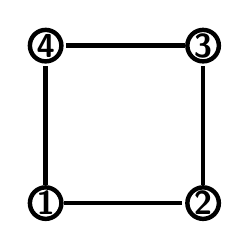
\begin{tikzpicture}[shorten >=1pt, auto, node distance=3cm, ultra thick,main node/.style={circle,draw,minimum size=.4cm,inner sep=0pt}]
\begin{scope}[every node/.style={font=\sffamily\large\bfseries}]
\node [main node](v1) at (0,0) {1};
\node [main node](v2) at (2,0) {2};
\node [main node](v3) at (2,2) {3};
\node [main node](v4) at (0,2) {4};
\end{scope}
\path 
	(v1) edge (v2)
    (v1) edge (v4)
    (v2) edge (v3)
    (v3) edge (v4)
         ;
\end{tikzpicture}
\caption*{$C_4$}
\end{figure}
\begin{figure}[H]
\centering
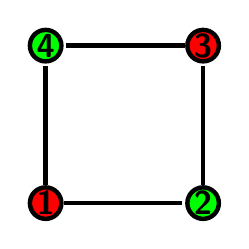
\begin{tikzpicture}[shorten >=1pt, auto, node distance=3cm, ultra thick,main node/.style={circle,draw,minimum size=.4cm,inner sep=0pt}]
\begin{scope}[every node/.style={font=\sffamily\large\bfseries}]
\node [main node,fill=red](v1) at (0,0) {1};
\node [main node,fill=green](v2) at (2,0) {2};
\node [main node,fill=red](v3) at (2,2) {3};
\node [main node,fill=green](v4) at (0,2) {4};
\end{scope}
\path 
	(v1) edge (v2)
    (v1) edge (v4)
    (v2) edge (v3)
    (v3) edge (v4)
         ;
\end{tikzpicture}
\caption*{I ,,Pokolorowane'' $C_4$}
\end{figure}
\begin{figure}[H]
\centering
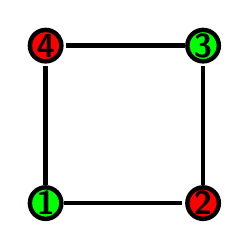
\begin{tikzpicture}[shorten >=1pt, auto, node distance=3cm, ultra thick,main node/.style={circle,draw,minimum size=.4cm,inner sep=0pt}]
\begin{scope}[every node/.style={font=\sffamily\large\bfseries}]
\node [main node,fill=green](v1) at (0,0) {1};
\node [main node,fill=red](v2) at (2,0) {2};
\node [main node,fill=green](v3) at (2,2) {3};
\node [main node,fill=red](v4) at (0,2) {4};
\end{scope}
\path 
	(v1) edge (v2)
    (v1) edge (v4)
    (v2) edge (v3)
    (v3) edge (v4)
         ;
\end{tikzpicture}
\caption*{II ,,Pokolorowane'' $C_4$}
\end{figure}
\end{multicols}
\begin{enumerate}[label=\alph*)]
\item Narysuj graf skierowany, obrazujący łańcuch Markowa odpowiadający podanemu algorytmowi. Zbiorem stanów powinny być wszystkie właściwe kolorowania grafu $G$.
\begin{figure}[H]
\centering
\begin{tikzpicture}[shorten >=1pt, auto, node distance=3cm, ultra thick,main node/.style={rectangle,draw,minimum size=.4cm,text width=3cm,text centered,rounded corners}]
\begin{scope}[every node/.style={font=\sffamily}]
\node (v0) at (-2.5,1.5) {START};
\node [main node](v1) at (0,0) {Wylosuj jeden z wierzchołków $v$};
\node [main node](v2) at (0,-2) {Wylosuj jeden z kolorów $i$};
\node [main node](v3) at (0,-4) {Czy kolorowanie jest właściwe?};
\node [main node](v4) at (-2,-6) {Przemaluj $v$ na $i$};
\node [main node](v5) at (2,-6) {Pozostaw bez zmian};

\end{scope}
\path 
	(v0) edge [->] node {} (v1)
	(v1) edge [->] node {$\sfrac{1}{4}$} (v2)
    (v2) edge [->] node[->] {$\sfrac{1}{2}$} (v3)
    (v3) edge [->] node {TAK} (v4)
    (v3) edge [->] node {NIE} (v5)
         ;
\end{tikzpicture}
\caption*{,,Pokolorowane'' $C_4$}
\end{figure}

Stany: $S:\{\{\text{I Pokolorowanie}\},\{\text{II Pokolorowanie}\}\}$
\begin{figure}[H]
\centering

\begin{tikzpicture}[shorten >=1pt, auto, node distance=3cm, ultra thick,main node/.style={rectangle,draw,minimum size=.4cm,inner sep=0pt}]
\begin{scope}[every node/.style={font=\sffamily}]
\node [main node](v1) at (0,0) {$\{\text{I Pokolorowanie}\}$};
\node [main node](v2) at (4,0) {$\{\text{II Pokolorowanie}\}$};
\end{scope}
\path 
	(v1) edge [loop above] node[near start] {$1$} (v1)
    (v2) edge [loop above] node[near start] {$1$} (v2)
         ;
\end{tikzpicture}
\end{figure}


\item Czy po bardzo dużej liczbie kroków każde właściwe kolorowanie będzie w przybliżeniu jednakowo prawdopodobne, niezależnie jaki był stan początkowy?

\textbf{Odpowiedź:} \textbf{NIE}, gdyż jak widać z rysunku diagramu powyżej, poszczególne stany łańcucha są pochłaniające - czytaj z stanu I nie przejdę do stanu II i vive versa. Czyli po bardzo dużej liczbie kroków prawdopodobieństwo będzie równe prawdopodobieństwu początkowemu. 
\end{enumerate}


\paragraph{A4} Generujemy lasy rozpięte grafu $K_3$ następująco. Zaczynamy od dowolnego lasu rozpiętego, a w każdym kroku, Mając wygenerowany las $H$, wybieramy z jednakowym prawdopodobieństwem jakąś krawędź z $E(K_3)$, a następnie rzucamy symetryczna, monetą.
\begin{figure}[H]
\centering
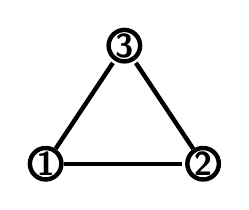
\begin{tikzpicture}[shorten >=1pt, auto, node distance=3cm, ultra thick,main node/.style={circle,draw,minimum size=.4cm,inner sep=0pt}]
\begin{scope}[every node/.style={font=\sffamily\large\bfseries}]
\node [main node](v1) at (0,0) {1};
\node [main node](v2) at (2,0) {2};
\node [main node](v3) at (1,1.5) {3};
\end{scope}
\path 
	(v1) edge (v2)
    (v1) edge (v3)
    (v2) edge (v3)
         ;
\end{tikzpicture}
\caption*{$K_3$}
\end{figure}
\begin{multicols}{4}[Możliwe lasy rozpięte na $K_3$]
Stan $I\ \rightarrow\ S_{I}$:\\
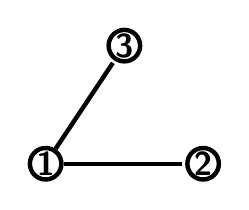
\begin{tikzpicture}[shorten >=1pt, auto, node distance=3cm, ultra thick,main node/.style={circle,draw,minimum size=.4cm,inner sep=0pt}]
\begin{scope}[every node/.style={font=\sffamily\large\bfseries}]
\node [main node](v1) at (0,0) {1};
\node [main node](v2) at (2,0) {2};
\node [main node](v3) at (1,1.5) {3};
\end{scope}
\path 
	(v1) edge (v2)
    (v1) edge (v3)
         ;
\end{tikzpicture}
Stan $II\ \rightarrow\ S_{II}$:\\
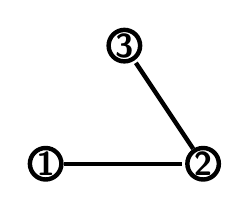
\begin{tikzpicture}[shorten >=1pt, auto, node distance=3cm, ultra thick,main node/.style={circle,draw,minimum size=.4cm,inner sep=0pt}]
\begin{scope}[every node/.style={font=\sffamily\large\bfseries}]
\node [main node](v1) at (0,0) {1};
\node [main node](v2) at (2,0) {2};
\node [main node](v3) at (1,1.5) {3};
\end{scope}
\path 
	(v1) edge (v2)
    (v2) edge (v3)
         ;
\end{tikzpicture}
Stan $III\ \rightarrow\ S_{III}$:\\
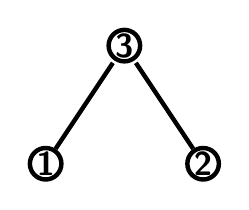
\begin{tikzpicture}[shorten >=1pt, auto, node distance=3cm, ultra thick,main node/.style={circle,draw,minimum size=.4cm,inner sep=0pt}]
\begin{scope}[every node/.style={font=\sffamily\large\bfseries}]
\node [main node](v1) at (0,0) {1};
\node [main node](v2) at (2,0) {2};
\node [main node](v3) at (1,1.5) {3};
\end{scope}
\path 
    (v1) edge (v3)
    (v2) edge (v3)
         ;
\end{tikzpicture}
Stan $IV\ \rightarrow\ S_{IV}$:\\
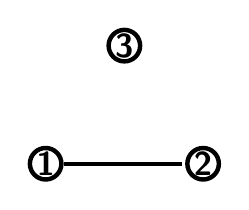
\begin{tikzpicture}[shorten >=1pt, auto, node distance=3cm, ultra thick,main node/.style={circle,draw,minimum size=.4cm,inner sep=0pt}]
\begin{scope}[every node/.style={font=\sffamily\large\bfseries}]
\node [main node](v1) at (0,0) {1};
\node [main node](v2) at (2,0) {2};
\node [main node](v3) at (1,1.5) {3};
\end{scope}
\path 
	(v1) edge (v2)
         ;
\end{tikzpicture}
Stan $V\ \rightarrow\ S_{V}$:\\
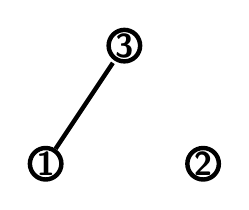
\begin{tikzpicture}[shorten >=1pt, auto, node distance=3cm, ultra thick,main node/.style={circle,draw,minimum size=.4cm,inner sep=0pt}]
\begin{scope}[every node/.style={font=\sffamily\large\bfseries}]
\node [main node](v1) at (0,0) {1};
\node [main node](v2) at (2,0) {2};
\node [main node](v3) at (1,1.5) {3};
\end{scope}
\path 
    (v1) edge (v3)
         ;
\end{tikzpicture}
Stan $VI\ \rightarrow\ S_{VI}$:\\
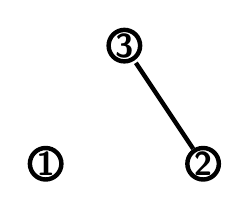
\begin{tikzpicture}[shorten >=1pt, auto, node distance=3cm, ultra thick,main node/.style={circle,draw,minimum size=.4cm,inner sep=0pt}]
\begin{scope}[every node/.style={font=\sffamily\large\bfseries}]
\node [main node](v1) at (0,0) {1};
\node [main node](v2) at (2,0) {2};
\node [main node](v3) at (1,1.5) {3};
\end{scope}
\path 
    (v2) edge (v3)
         ;
\end{tikzpicture}
Stan $VII\ \rightarrow\ S_{VII}$:\\
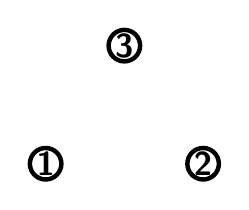
\begin{tikzpicture}[shorten >=1pt, auto, node distance=3cm, ultra thick,main node/.style={circle,draw,minimum size=.4cm,inner sep=0pt}]
\begin{scope}[every node/.style={font=\sffamily\large\bfseries}]
\node [main node](v1) at (0,0) {1};
\node [main node](v2) at (2,0) {2};
\node [main node](v3) at (1,1.5) {3};
\end{scope}
\end{tikzpicture}
\end{multicols}
\begin{itemize}
\item Jeżeli wypadł orzeł i wybrana krawędź należy do lasu $H$, to ją usuwamy.
\item Jeżeli wypadła reszka i wybrana krawędź nie należy do $H$, to dodajemy ją do $H$ (o ile nie domyka cyklu).
\item W przeciwnym wypadku nic nie robimy.
\end{itemize}
Budujemy łańcuch Markowa odpowiadający powyższemu algorytmowi, w którym stanami są wszystkie lasy rozpięte w $K_3$.
\begin{enumerate}[label=\alph*)]
\item Ile stanów ma ten łańcuch?

\textbf{Odpowiedź:} Łańcuch ma 7 stanów: $S=\{S_{I},S_{II},S_{III},S_{IV},S_{V},S_{VI},S_{VII},\}$
\item Proszę wybrać w $K_3$ drzewo rozpięte i podać wiersz macierzy przejścia łańcucha, odpowiadający temu stanowi.

\begin{align*}
&S_{I}\rightarrow S_{I}   & \frac{1}{2}*\frac{1}{3}+\frac{1}{2}=\frac{2}{3} &\text{ Orzeł i krawędź 2-3 albo Reszka}\\
&S_{I}\rightarrow S_{II}  & 0 &\text{ Nie da się w jednym kroku przejść z I do II}\\
&S_{I}\rightarrow S_{III} & 0 &\text{ Nie da się w jednym kroku przejść z I do III}\\
&S_{I}\rightarrow S_{IV}  & \frac{1}{2}*\frac{1}{3}=\frac{1}{6} &\text{ Orzeł i krawędź 1-3}\\
&S_{I}\rightarrow S_{V}   & \frac{1}{2}*\frac{1}{3}=\frac{1}{6} &\text{ Orzeł i krawędź 1-2}\\
&S_{I}\rightarrow S_{VI}  & 0 &\text{ Nie da się w jednym kroku przejść z I do VI}\\
&S_{I}\rightarrow S_{VII} & 0 &\text{ Nie da się w jednym kroku przejść z I do VII}
\end{align*}

$$\bar{P}(S_I)=\bbordermatrix{&S_{I}&S_{II}&S_{III}&S_{IV}&S_{V}&S_{VI}&S_{VII} \cr
S_I& \sfrac{2}{3} &0&0&\sfrac{1}{6}&\sfrac{1}{6}&0&0}$$
\item Czy łańcuch jest ergodyczny?

\textbf{Odpowiedź: }Gdybym napisał całą macierz, pewnie by wyszło, że z każdego stanu do każdego innego stanu bezpośrednio albo pośrednio mogę przejść.
\item Czy łańcuch jest odwracalny?

\textbf{Odpowiedź: }\textbf{CHYBA }Tak, gdyż zgodnie z definicja Odwracalności (\ref{def:OdwracalnoscLM2} na stronie \pageref{def:OdwracalnoscLM2}) gdybym zrobił całą macierz i wyliczył wektor własny, to by chyba wyszło.
\end{enumerate}

\paragraph{A5} Generujemy lasy rozpięte grafu $G$ następująco. Zaczynamy od dowolnego lasu rozpiętego, a w każdym kroku, Mając wygenerowany las $H$, wybieramy jednostajnie krawędź z $E(G)$ i z prawdopodobieństwem $\frac{1}{2}$ usuwamy ją z $H$ (Jeśli nie jest ona krawędzią $H$, to nic nie robimy), a z prawdopodobieństwem $\frac{1}{2}$ dodajemy ją do $H$ (o ile nie domyka cyklu).
\begin{enumerate}[label=\alph*)]
\item Czy łańcuch jest odwracalny?

\textbf{Odpowiedź: }Tak, Dowód przedstawiony w zadaniu \ref{par:10-A2} (strona \pageref{par:10-A2})
\item Czy jest ergodyczny?

\textbf{Odpowiedź: }Tak, Dowód przedstawiony w zadaniu \ref{par:10-A2} (strona \pageref{par:10-A2})
\item Czy możemy stwierdzić, że po wielu krokach każdy las rozpięty będzie w przybliżeniu jednakowo prawdopodobny?

\textbf{Odpowiedź: }Tak, Dowód przedstawiony w zadaniu \ref{par:10-A2} (strona \pageref{par:10-A2})
\end{enumerate}

\subsection{Zadania domowe B}
\paragraph{B1} Tasujemy talię $n$ ($n \geq 2$) kart w taki sposób: zaczynamy od dowolnego stosu, wybieramy losowo (z jednakowym prawdopodobieństwem) jedną z $n$ kart i kładziemy ją na wierzch.
\begin{enumerate}[label=\alph*)]
\item Sprawdź, że rozkład jednostajny jest rozkładem stacjonarnym tego łańcucha.
\item Uzasadnij, że łańcuch jest nieokresowy i nieprzywiedlny.
\item Czy po wielu krokach uzyskamy każde potasowanie z prawdopodobieństwem w przybliżeniu jednakowym?
\end{enumerate}

\paragraph{B2} Zaproponuj algorytm oparty na łańcuchu Markowa o $2^k$ stanach, który po wielu krokach wygeneruje każdy wierzchołek $k$-kostki z prawdopodobieństwem w przybliżeniu jednakowym. Zakładamy, że $k$ jest duże i stworzenie listy wszystkich $2^k$ wierzchołków $k$-kostki jest nieekonomiczne.

\paragraph{B3} Opisz zwięźle ideę algorytmu, generującego losowe skojarzenia w grafie (w tym zbiór pusty), w taki sposób, by każde ze skojarzeń $M$ wylosowane zostało z prawdopodobieństwem
\begin{enumerate}[label=\alph*)]
\item prawie jednakowym.
\item  bliskim
$$\frac{5^{|M|}}{\sum _S 5^{|S|}}$$
gdzie $|M|$ jest liczbą krawędzi w skojarzeniu $M$, a suma w mianowniku przebiega wszystkie skojarzenia
grafu (i zbiór pusty).
\item bliskim 
$$\frac{1}{3^{|M|*\sum _S\left(\sfrac{1}{3}\right)^{|S|}}}$$
gdzie $|M|$ jest liczbą krawędzi w skojarzeniu $M$, a suma w mianowniku przebiega wszystkie skojarzenia
grafu (i zbiór pusty). 
\end{enumerate}
Najważniejszą częścią tego zadania jest uzasadnienie poprawności algorytmu.

\paragraph{B4} Graf $G$ na $4$ wierzchołkach, będący cyklem z przekątną. Mamy też 3 kolory (czyli mniej niż $\Delta + 2$). Generujemy wszystkie właściwe kolorowania wierzchołków grafu $G$ następująco:
\begin{itemize}
\item Mając kolorowanie właściwe, wylosuj jeden z czterech wierzchołków $v$, każdy z jednakowym prawdopodobieństwem i wylosuj jeden z trzech kolorów $i$, każdy z jednakowym prawdopodobieństwem.
\item Jeśli po przemalowaniu wierzchołka $v$ na kolor $i$ kolorowanie pozostaje właściwe, przemaluj $v$ na kolor $i$.
\item W przeciwnym przypadku pozostaw kolorowanie bez zmian.
\end{itemize}
\begin{enumerate}[label=\alph*)]
\item Narysuj graf skierowany, obrazujący łańcuch Markowa odpowiadający podanemu algorytmowi. Zbiorem
stanów powinny być wszystkie właściwe kolorowania grafu $G$.
\item Czy po bardzo dużej liczbie kroków każde właściwe kolorowanie będzie w przybliżeniu jednakowo prawdopodobne, niezależnie jaki był stan początkowy?
\end{enumerate}


\paragraph{B5} Mamy $3$ kolory i graf $G = C_4$, czyli będący cyklem o $4$ wierzchołkach. Generujemy wszystkie właściwe kolorowania wierzchołków grafu $G$ następująco:
\begin{itemize}
\item Mając kolorowanie właściwe, wylosuj jeden z wierzchołków $v$, każdy z jednakowym prawdopodobieństwem i wylosuj jeden z kolorów $i$, każdy z jednakowym prawdopodobieństwem.
\item Jeśli po przemalowaniu wierzchołka $v$ na kolor $i$ kolorowanie pozostaje właściwe, przemaluj $v$ na kolor $i$.
\item W przeciwnym przypadku pozostaw kolorowanie bez zmian.
\end{itemize}
\begin{enumerate}[label=\alph*)]
\item Ile stanów ma łańcuch Markowa odpowiadający podanemu algorytmowi? Zbiorem stanów powinny być
wszystkie właściwe kolorowania grafu $G$.
\item Wyznacz pierwszy wiersz macierzy przejścia tego łańcucha (stan numer jeden wybierz samodzielnie).
\item Czy po bardzo dużej liczbie kroków każde właściwe kolorowanie będzie w przybliżeniu jednakowo prawdopodobne, niezależnie jaki był stan początkowy?
\item Jeśli w poprzednim podpunkcie zapomniałeś sprawdzić, czy łańcuch jest ergodyczny, zrób to teraz.
\end{enumerate}


\paragraph{B6} Mamy $n$ przedmiotów, o objętościach odpowiednio $v_1, . . . , v_n$. Mamy też plecak o pojemności $b$. Plecak możemy zapakować wybierając dowolnie zestaw przedmiotów (w tym zestaw pusty), o ile suma ich objętości nie przekracza pojemności plecaka. Zaproponuj algorytm oparty na łańcuchu Markowa, który po wielu krokach wybierze zestaw przedmiotów możliwy do zapakowania w taki sposób, by przybliżone prawdopodobieństwo wylosowania zestawu było funkcją rosnącą liczby przedmiotów w zestawie. Najważniejszą częścią zadania jest uzasadnienie poprawności algorytmu.

\paragraph{B7 *} Na wykładzie został tak zdefiniowany łańcuch Markowa na rodzinie wszystkich zbiorów niezależnych grafu, że współrzędne rozkładu stacjonarnego były proporcjonalne wykładniczo do rozmiaru zbioru. Skonstruuj łańcuch Markowa na rodzinie wszystkich zbiorów niezależnych grafu w taki sposób, aby współrzędne rozkładu stacjonarnego były proporcjonalne liniowo do rozmiaru zbioru.

\subsection{Zadania}
\paragraph{Zad.1} Wygeneruj za pomocą łańcucha Markowa o $2^n$ stanach wszystkie podzbiory zbioru $n$– elementowego tak, aby
\begin{enumerate}[label=\alph*)]
\item w rozkładzie stacjonarnym dla tego procesu wszystkie podzbiory były jednakowo prawdopodobne.
\item po wielu krokach otrzymać każdy podzbiór z prawdopodobieństwem w przybliżeniu jednakowym.
\item przybliżone prawdopodobieństwo wylosowania zbioru było funkcją rosnącą jego rozmiaru.
Zakładamy, że $n$ jest duże i stworzenie listy wszystkich $2^n$ podzbiorów jest nieekonomiczne.
\end{enumerate}

\paragraph{Zad.2} Lisek Chytrusek zaproponował poniższy algorytm (oparty na łańcuchu Markowa) do dobrego potasowania 52 kart. Celem liska było stworzyć algorytm, który po wielu krokach (np. 100tys) wygeneruje każde potasowanie z prawdopodobieństwem w przybliżeniu jednakowym. Algorytm liska: Zaczynam od dowolnego potasowania. W każdym kroku wybieram losowo kolejno dwie, niekoniecznie różne, karty (każdą losuję jednostajnie) i zamieniam miejscami. Sprawdź poprawność algorytmu.

\paragraph{Zad.3} Oto znany problem plecakowy. Mamy $n$ przedmiotów, o objętościach odpowiednio $v_1, . . . , v_n$. Mamy też plecak o pojemności $b$. Plecak możemy zapakować wybierając dowolnie zestaw przedmiotów (w tym zestaw pusty), o ile suma ich objętości nie przekracza pojemności plecaka. Zaproponuj algorytm oparty na łańcuchu Markowa, który po wielu krokach wybierze zestaw przedmiotów możliwy do zapakowania w sposób w przybliżeniu jednostajny (tzn. każdy zestaw będzie z grubsza jednakowo prawdopodobny).
